Our results are organized as follows.
%
Sections~\ref{sec:nyx} and\ref{sec:sw4} present findings from our study investigating reduced Lagrangian representations for cosmology and seismology applications, respectively.
%
%Section~\ref{sec:cloverleaf3d} contains results from our benchmarking study.
%
%We organize our results by discussing the use of Lagrangian representations for the cosmology and seismology () applications, and  .
%
Tables~\ref{table:nyx_encumbrance} and~\ref{table:sw4_encumbrance} provide information pertaining to in situ encumbrance experiments, such as concurrency information, spatial dimensions, Sim$_{cycle}$, number of particles, \textbf{InSituMem}, \textbf{Step}, and \textbf{DAV\%}, for each application. 
%
Figure~\ref{fig:insitucost} contains the execution time per cycle for all the in situ encumbrance experiments. %from both applications.  
%
\begin{figure}[!b]
\centering
\vspace{-4mm}
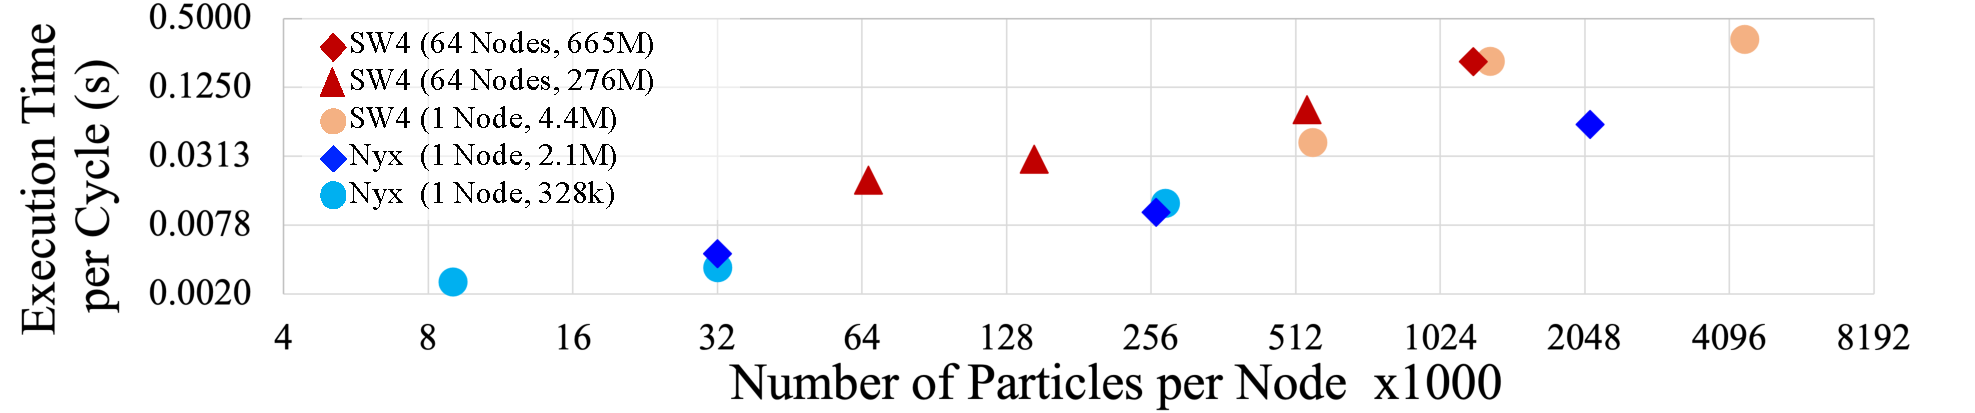
\includegraphics[width=\linewidth]{Images/InSituCost_Stretch2.pdf}
%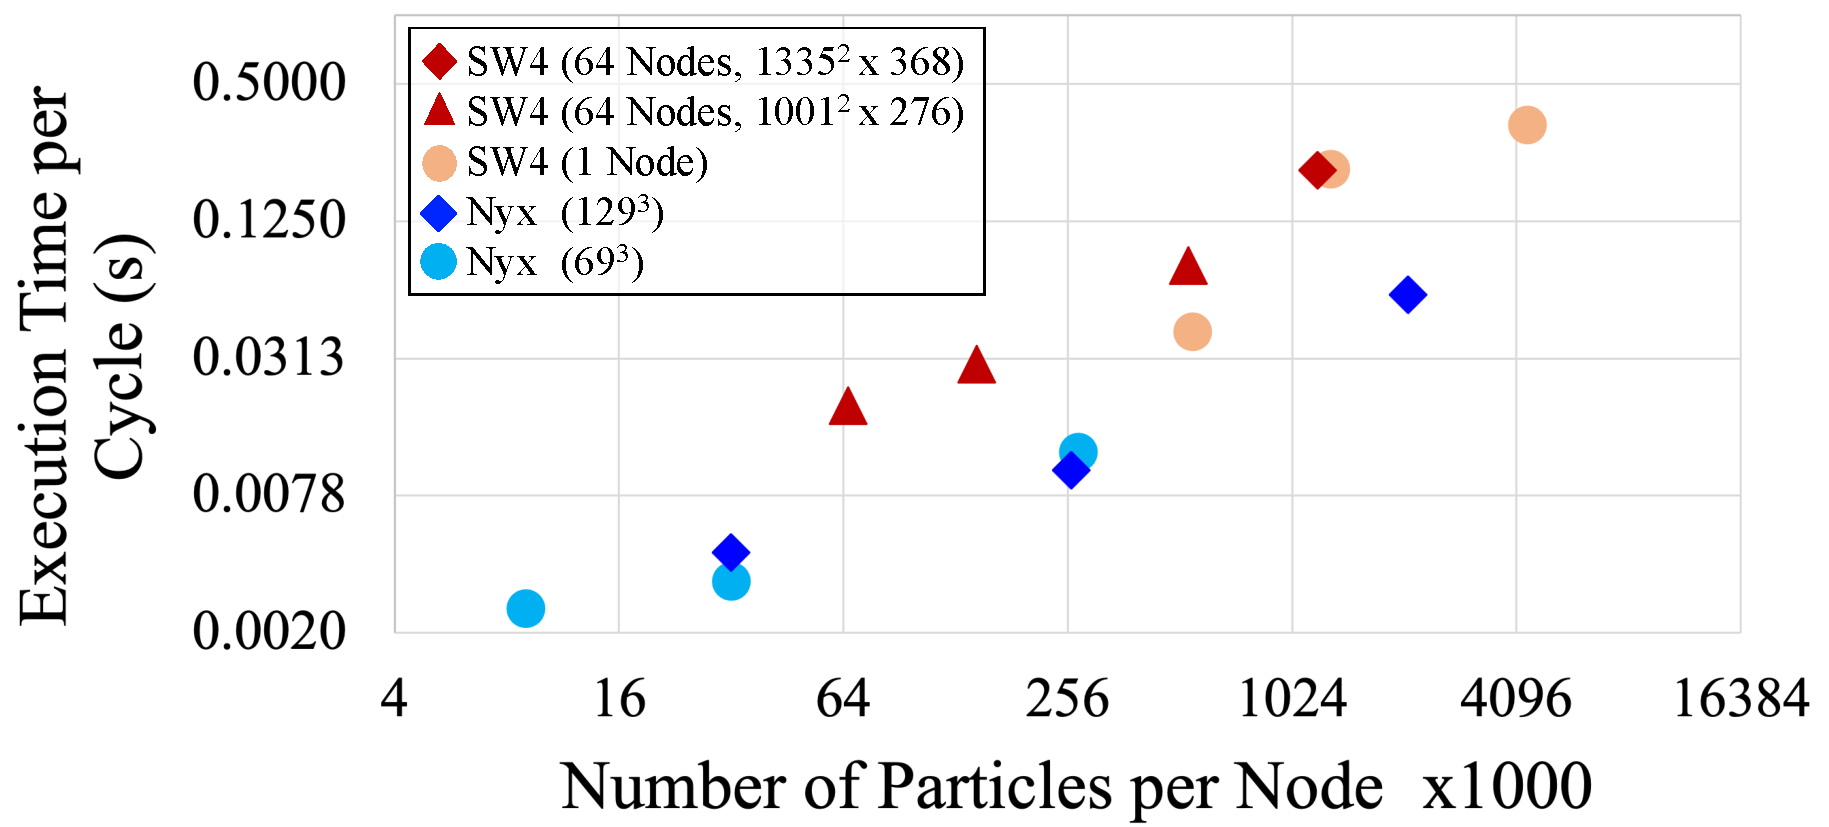
\includegraphics[width=0.7\linewidth]{Images/InSituCost.pdf}
\vspace{-5mm}
\caption{Lagrangian in situ reduction cost per cycle for all in situ encumbrance experiments. The SW4 simulation executes with six ranks (each allocated one GPU) sharing memory on every node. The Nyx simulation executes on a single rank using all the cores of two CPUs on a single node. The legend includes concurrency and number of simulation grid points in parenthesis and both axes use logarithmic scales.} 
\vspace{-5mm}
\label{fig:insitucost}
\end{figure}

%
Figures~\ref{fig:nyx_violinplot},~\ref{fig:nyx_figure},~\ref{fig:sw4_violinplot}, and ~\ref{fig:sw4_figure} show the results of our post hoc efficacy evaluation.
%
For each application, the figures are annotated with configuration specifics such as the \textbf{DS}, \textbf{1:X}, and \textbf{I}.
%
Further, Lagrangian and Eulerian tests are distinguished explicitely in the captions or are labeled L$T$ and E$T$, respectively, where $T$ is the test number.
%
%We refer to these tables and figures in the discussion that follows. 

\vspace{-1mm}
\subsection{Nyx Cosmology Simulation}
\label{sec:nyx}
\noindent\textbf{In Situ Encumbrance}
Using all the cores of two CPUs on a single compute node, we used OpenMP to parallelize the Nyx simulation and Lagrangian VTK-m filter.
%
We tested two options for grid size - $69^{3}$ and $129^{3}$ - on a single rank, and three particle advection workloads (1:1, 1:8, 1:27) each.
%
In a single compute node hour, the simulation performed approximately 300 and 38 cycles, when using $69^{3}$ and $129^{3}$ grid sizes, respectively.
%
%In a single compute node hour, the simulation performs approximately 300 cycles for the $69^{3}$ resolution and approximately 38 cycles for the $129^{3}$ resolution.
%
An 8X increase in grid size results in a proportional increase in Sim$_{cycle}$ but only a small increase in particle advection costs for the same number of particles.
%
We expect a single rank to operate on between $32^{3}$ to $256^{3}$ grid resolutions, and thus our workloads provide a representative estimate of \textbf{DAV\%}.
%
%For example, sampling a $256^{3}$ using a 1:8 reduction involves computing 2.1M basis trajectories. 

An encouraging finding is the low in situ encumbrance when performing L-ISR on the CPUs.
%
Depending on the setup of various simulations and the form of integration for in situ processing, future work can consider offloading L-ISR computation to CPUs.
%
Overall, considering the longer Sim$_{cycle}$ times for the Nyx simulation, and parallel compution coupled with low memory latency when using CPUs, the highest in situ encumbrance to extract a Lagrangian represenation was 0.1\% of the simulation time or under 0.06s to compute 2.1M basis trajectories per cycle.\\
\begingroup
\setlength{\tabcolsep}{-2pt}
%\renewcommand{\arraystretch}{1} % Default value: 1
\begin{table*}[!t]
%\centering
\begin{tabular}{|P{1.1cm}|P{1.1cm}|P{2.7cm}|P{1.3cm}|P{1.5cm}|P{1.9cm}|P{1.7cm}|P{1.7cm}|}
\hline
Nodes & Ranks & Dimensions & \textbf{Sim$_{cycle}$} & Particles & \textbf{InSituMem} & \textbf{Step} & \textbf{DAV\%} \\ 
% & Ranks & & & /Node & /Node (MB) & & \\ 
\hline
%\multicolumn{9}{l}{} & \\
%\multicolumn{9}{l}{\textbf{          Cloverleaf3D Proxy Hydrodynamics Application }} \\ %& \multirow{13}{*}{\includegraphics[width=0.93\linewidth]{images/GPU_Step.pdf}}\\
%\cline{1-9}
%\multirow{9}{*}{16} & \multirow{9}{*}{96} & \multirow{9}{*}{$586\times586\times586$} & 20 & 4.73 & \multirow{3}{*}{1.5M} & \multirow{3}{*}{40.2 } & 0.4475 & 9.408 \\
%\cline{4-4}
%& & & 40 & 4.08 & & & 0.3221 & 7.894 \\
%\cline{4-4}
%& & & 60 & 4.39 & & & 0.3838 & 8.742 \\
%\cline{4-6}%\cline{6-6}
%& & & 20 & 4.50 & \multirow{3}{*}{474k} & \multirow{3}{*}{12 } & 0.1882 & 4.182 \\
%\cline{4-4}
%& & & 40 & 4.14 & & & 0.1628 & 3.932 \\
%\cline{4-4}
%& & & 60 & 4.33 & & & 0.1498 & 3.459 \\
%\cline{4-6}%\cline{6-6}
%& & & 20 & 4.19 & \multirow{3}{*}{186k} & \multirow{3}{*}{4.2 } & 0.0925 & 2.207 \\
%\cline{4-4}
%& & & 40 & 4.11 & & & 0.1043 & 2.537 \\
%\cline{4-4}
%& & & 60 & 3.87 & & & 0.0830 & 2.144 \\
%\cline{1-9}
%%\multicolumn{9}{l}{} & \\
%\multicolumn{8}{l}{\textbf{          SW4 Seismic Modeling Simulation }}\\
%\cline{1-8}
%\multirow{3}{*}{1} & \multirow{3}{*}{6} & $251\times251\times70$ & 0.35s & 555k & 13.89MB & 0.0412s & 11.67\% \\
%%\cline{3-3}\cline{5-6}
%& & $335\times335\times93$  & 2.02s & 1.3M & 33.16MB & 0.2125s & 10.48\% \\
%%\cline{3-3}\cline{5-6}  
%& & $501\times501\times139$  & 7.58s & 4.4M & 111.13MB & 0.3309s & 4.365\% \\ %& \multirow{13}{*}{\includegraphics[width=0.93\linewidth]{images/CPU_Step.pdf}}\\
%\cline{1-3}%\cline{5-6}
%\multirow{4}{*}{64} & \multirow{4}{*}{384} & \multirow{3}{*}{$1001\times1001\times276$} & 1.6s & 66k & 1.6MB & 0.0194s & 1.201\% \\
%%\cline{6-6}
%& & & 1.5s & 146k & 3.6MB & 0.0295s & 1.944\% \\
%%\cline{6-6}
%& & & 1.3s & 540k & 13.5MB & 0.0798s & 6.175\% \\
%\cline{3-3}%\cline{5-6}
%& & $1335\times1335\times368$ & 2.9s & 1.2M & 31.9MB & 0.2095s & 7.074\% \\
%\cline{1-8}
%%\multicolumn{9}{l}{} \\
%\multicolumn{8}{l}{\textbf{          Nyx Cosmology Simulation }} \\
\cline{1-8}
\multirow{6}{*}{1} & \multirow{6}{*}{1} & \multirow{3}{*}{$65\times65\times65$} & \multirow{3}{*}{10.9s} & 9k & 0.2MB & 0.0025s & 0.023\% \\
%\cline{6-6}
& & & & 32k & 0.8MB & 0.0033s & 0.030\% \\
%\cline{6-6}
& & & & 274k & 6.8MB & 0.0122s & 0.0112\% \\
\cline{3-3}%\cline{5-6}
& & \multirow{3}{*}{$129\times129\times129$} & \multirow{3}{*}{88.3s} & 78k & 1.9MB & 0.0044s & 0.005\% \\
%\cline{6-6}
& & & & 262k & 6.5MB & 0.0101s & 0.011\% \\
%\cline{6-6}
& & & & 2.1M & 53.6MB & 0.0596s & 0.067\% \\
\hline
\end{tabular}
\caption{\textit{In situ} encumbrance evaluation and experiment configurations for the Nyx simulation executing on CPUs. The in situ cost of computing Lagrangian representations every cycle~(\textbf{Step}) remains low in comparison to the average simulation cycle time~(\textbf{Sim$_{cycle}$}) resulting in low \textbf{DAV\%}.}
\vspace{-5mm}
\label{table:nyx_encumbrance}
\end{table*}
\endgroup

\begin{figure}[!t]
\centering
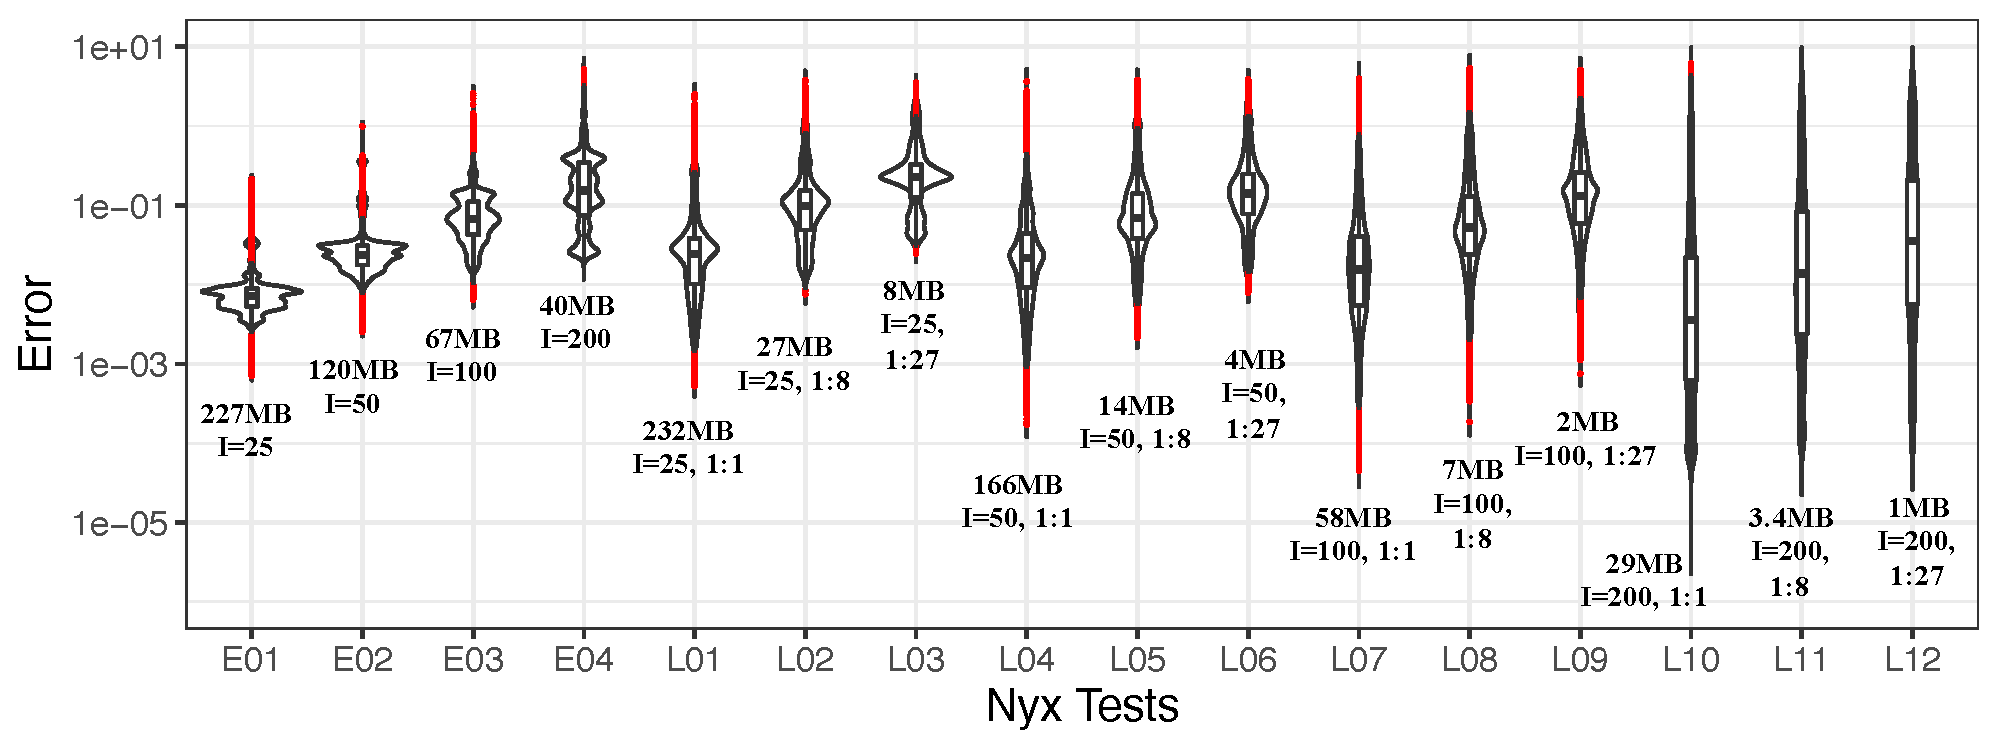
\includegraphics[width=\linewidth]{Images/nyx_violinplot.pdf}
\vspace{-5mm}
\caption{Efficacy results for the Nyx experiments. Each violin plot shows the distribution of the particle reconstruction error for a specific configuration and the horizontal blue dashed line in the chart represents an error equivalent to a single grid cell side. While Eulerian configurations contain greater uncertainty as the value of storage interval \textbf{I} increases, the Lagrangian representations offer the opportunity for improvements in accuracy. Additionally, we find high reconstruction accuracy relies on a high spatial sampling resolution as well.}
\label{fig:nyx_violinplot}
\end{figure}

\begin{figure}[!t]
\centering
\includegraphics[width=\linewidth]{Images/nyx_figure.pdf}
\vspace{-5mm}
\caption{Pathline visualization of baryonic particles evolution in self-gravitating gas dynamics of Nyx simulation. Using 10,000 randomly seeded particles, we visualize pathlines over 300 cycles. To focus on regions where particles cluster to form dense regions, we set opacity of the pathline to be directly proportional to time. Thus, we are able to focus on clustering as well as provide context of transport toward these regions. Lagrangian representations are able to reconstruct the ground truth trajectories and capture clustering accurately when a high spatial sampling is used~(1:1, 1:8). However, when using a 1:27 data reduction factor, some clusters are visualized less clearly.} 
\vspace{-5mm}
\label{fig:nyx_figure}
\end{figure}


\noindent\textbf{Post Hoc Efficacy}
To evaluate the usefulness of Lagrangian representations to encode time-varying self-gravitating gas dynamics, we considered three options for data reduction (1:1, 1:8, 1:27) and four options for \textbf{I}~(25, 50, 100, 200).
%
We constructed pathlines for 50,000 randomly placed particles over 400 cycles during post hoc analysis.
%
%We measure the error of reconstruction of each pathline by comparing to ground truth trajectories.
%
%Additionally, we compute pathlines using Eulerian representations at full spatial resolution and same options for \textbf{I}.
%
We visualize the distribution of reconstruction error for all tests in Figure~\ref{fig:nyx_violinplot}.
%We measure the error or reconstruction of each pathline. and visualize the distribution in Figure~\ref{} along with  
%

The self-gravitating gas dynamics of this simulation produce a vector field that captures the transport of randomly distributed particles to multiple high-density clusters.
%
Particles travel with increasing velocity as clusters increase in density.
%
For this data, we found that Eulerian temporal subsampling performs better for small values of \textbf{I}.
%
This result can be expected given reconstruction using an Eulerian representation and fourth-order Runge Kutta interpolation remain more accurate than second-order barycentric coordinates interpolation employed to interpolate Lagrangian representations~\cite{bujack2015lagrangian}\cite{hummel2016error}.
%
%This can be expected for two reasons: 1) for small values of \textbf{I}, trajectories computed using fourth-order RK4 and Eulerian representations can remain more accurate than second-order barycentric coordinates interpolation and Lagrangian representations (although these are computed in situ using fourth-order RK4), and 2) use of several short Lagrangian flow maps can result in a higher error propagation and accumulation~\cite{bujack2015lagrangian,hummel2016error}.
%
However, as the value of \textbf{I} increases, the distribution of error for the Lagrangian tests indicates that a larger percentage of samples are reconstructed more accurately.
%
The Lagrangian representation computed in situ using RK4 encodes the behavior over an interval of time more accurately for the majority of samples.
%
In contrast, Eulerian representations become less effective at reconstructing the vector field due to increased numerical approximation and accumulating error.
%
%With regard to spatial sampling resolution, for the grid size we consider, we find that reducing the number of samples has a considerable impact on the efficacy of reconstruction.
%
%This indicates that small changes in starting location can result in particles transporting to different clusters.
%

We used pathlines with manually set transfer functions to visualize the evolution and clustering of particles in regions of high density.
%
The total size of the simulation vector field data used to compute the ground truth is 5.3GB.
%
We visualize a random subset of 10,000 pathlines in Figure~\ref{fig:nyx_figure} for configurations with \textbf{I} set to 25.
%To visualize the evolution and clustering of particles in regions of high density, we visualize a random subset of 10,000 pathlines in Figure~\ref{fig:nyx_figure} for configurations with \textbf{I} set to 25.
%
We note that Lagrangian configurations (L04 to L12) using larger values of \textbf{I} are more accurate statistically~(Figure~\ref{fig:nyx_violinplot}).
%
%
The Lagrangian representations demonstrate the ability to closely reconstruct regions where dense clusters are formed while requiring a fraction of the total simulation data size.
%
For example, the 1:8 Lagrangian configuration enables the visualization of transport to dense clusters while requiring only 27MB, i.e., a 200X data reduction of the uncompressed vector field.
%

\vspace{-1mm}
\subsection{SW4 Seismology Simulation}
\label{sec:sw4}
\noindent\textbf{In Situ Encumbrance}
For the SW4 simulation, we considered five grid sizes at varying concurrencies.
%
In each case, we used all six GPUs available on a compute node to execute the simulation and L-ISR.
%
For all L-ISR workloads tested, the execution time required per cycle remained under 0.5 seconds on average, and the maximum in situ memory required by a node was 112 MB to compute the trajectories for 4.4M particles.
%
The cost for performing L-ISR was most dependent on the number of particles and only slightly impacted by increasing grid sizes.
%
%Figure~\ref{fig:insitucost} provides insight regarding performance using GPUs and CPUs. 
%
Referencing Figure~\ref{fig:insitucost}, although the SW4 experiments used six GPUs, we found execution time to be slower than Nyx experiments due to the use of shared memory by multiple ranks~(each has its own data block) and the high cost of launching kernels on the GPU for limited amounts of computation~(each basis particle advances by only a single step/cycle each invocation). 
%
%Increasing grid sizes, however, typically result in longer \textbf{Sim$_{cycle}$} times, and thus, lower \textbf{DAV\%}.
%
%
%DAV\% was closely related to both the Sim$_{cycle}$ and \textbf{Step} cost.
%
%Using fixed concurrency, fixed data reduction factor, and varying grid sizes, we observed \textbf{DAV\%} decrease from 11.67\% to 4.365\% as the grid size increased.
%
%Using fixed concurrency, fixed grid size, and varying data reduction factor, we observed \textbf{DAV\%} increase from 1.201\% to 6.175\% as the number of particles increased.
%
\begingroup
\setlength{\tabcolsep}{-2pt}
%\renewcommand{\arraystretch}{1} % Default value: 1
\begin{table*}[!b]
%\centering
\begin{tabular}{|P{1.1cm}|P{1.1cm}|P{2.7cm}|P{1.3cm}|P{1.5cm}|P{1.9cm}|P{1.7cm}|P{1.7cm}|}
\hline
Nodes & Ranks & Dimensions & \textbf{Sim$_{cycle}$} & Particles & \textbf{InSituMem} & \textbf{Step} & \textbf{DAV\%} \\ 
% & Ranks & & & /Node & /Node (MB) & & \\ 
\hline
%\multicolumn{9}{l}{} & \\
%\multicolumn{9}{l}{\textbf{          Cloverleaf3D Proxy Hydrodynamics Application }} \\ %& \multirow{13}{*}{\includegraphics[width=0.93\linewidth]{images/GPU_Step.pdf}}\\
%\cline{1-9}
%\multirow{9}{*}{16} & \multirow{9}{*}{96} & \multirow{9}{*}{$586\times586\times586$} & 20 & 4.73 & \multirow{3}{*}{1.5M} & \multirow{3}{*}{40.2 } & 0.4475 & 9.408 \\
%\cline{4-4}
%& & & 40 & 4.08 & & & 0.3221 & 7.894 \\
%\cline{4-4}
%& & & 60 & 4.39 & & & 0.3838 & 8.742 \\
%\cline{4-6}%\cline{6-6}
%& & & 20 & 4.50 & \multirow{3}{*}{474k} & \multirow{3}{*}{12 } & 0.1882 & 4.182 \\
%\cline{4-4}
%& & & 40 & 4.14 & & & 0.1628 & 3.932 \\
%\cline{4-4}
%& & & 60 & 4.33 & & & 0.1498 & 3.459 \\
%\cline{4-6}%\cline{6-6}
%& & & 20 & 4.19 & \multirow{3}{*}{186k} & \multirow{3}{*}{4.2 } & 0.0925 & 2.207 \\
%\cline{4-4}
%& & & 40 & 4.11 & & & 0.1043 & 2.537 \\
%\cline{4-4}
%& & & 60 & 3.87 & & & 0.0830 & 2.144 \\
%\cline{1-9}
%%\multicolumn{9}{l}{} & \\
%%\multicolumn{8}{l}{\textbf{          SW4 Seismic Modeling Simulation }}\\
\cline{1-8}
\multirow{3}{*}{1} & \multirow{3}{*}{6} & $251\times251\times70$ & 0.35s & 555k & 13.89MB & 0.0412s & 11.67\% \\
%\cline{3-3}\cline{5-6}
& & $335\times335\times93$  & 2.02s & 1.3M & 33.16MB & 0.2125s & 10.48\% \\
%\cline{3-3}\cline{5-6}  
& & $501\times501\times139$  & 7.58s & 4.4M & 111.13MB & 0.3309s & 4.365\% \\ %& \multirow{13}{*}{\includegraphics[width=0.93\linewidth]{images/CPU_Step.pdf}}\\
\cline{1-3}%\cline{5-6}
\multirow{4}{*}{64} & \multirow{4}{*}{384} & \multirow{3}{*}{$1001\times1001\times276$} & 1.6s & 66k & 1.6MB & 0.0194s & 1.201\% \\
%\cline{6-6}
& & & 1.5s & 146k & 3.6MB & 0.0295s & 1.944\% \\
%\cline{6-6}
& & & 1.3s & 540k & 13.5MB & 0.0798s & 6.175\% \\
\cline{3-3}%\cline{5-6}
& & $1335\times1335\times368$ & 2.9s & 1.2M & 31.9MB & 0.2095s & 7.074\% \\
\cline{1-8}
%\multicolumn{9}{l}{} \\
%\multicolumn{8}{l}{\textbf{          Nyx Cosmology Simulation }} \\
%\cline{1-8}
%\multirow{6}{*}{1} & \multirow{6}{*}{1} & \multirow{3}{*}{$65\times65\times65$} & \multirow{3}{*}{10.9s} & 9k & 0.2MB & 0.0025s & 0.023\% \\
%%\cline{6-6}
%& & & & 32k & 0.8MB & 0.0033s & 0.030\% \\
%%\cline{6-6}
%& & & & 274k & 6.8MB & 0.0122s & 0.0112\% \\
%\cline{3-3}%\cline{5-6}
%& & \multirow{3}{*}{$129\times129\times129$} & \multirow{3}{*}{88.3s} & 32k & 0.8MB & 0.0044s & 0.005\% \\
%%\cline{6-6}
%& & & & 262k & 6.5MB & 0.0101s & 0.011\% \\
%%\cline{6-6}
%& & & & 2.1M & 53.6MB & 0.0596s & 0.067\% \\
\hline
\end{tabular}
\caption{In situ encumbrance evaluation and experiment configurations for the SW4 simulation executing on GPUs. Overall, the \textbf{DAV\%} depends on the number of grid points per rank, the number of particles, i.e., the spatial sampling resolution, as well as the \textbf{Sim$_{cycle}$}.}
%We find \textbf{Sim$_{cycle}$} is more sensitive to the grid dimensions than the cost to perform L-ISR. As the grid dimensions increase, the \textbf{Sim$_{cycle}$} increases and thus, \textbf{DAV\%} decreases. For a fixed grid size, the \textbf{DAV\%} is directly proportional to the spatial sampling resolution, i.e., the number of particles.}
\label{table:sw4_encumbrance}
\end{table*}
\endgroup


\begin{figure}[!b]
\vspace{-5mm}
\begin{subfigure}{0.495\textwidth}
\centering
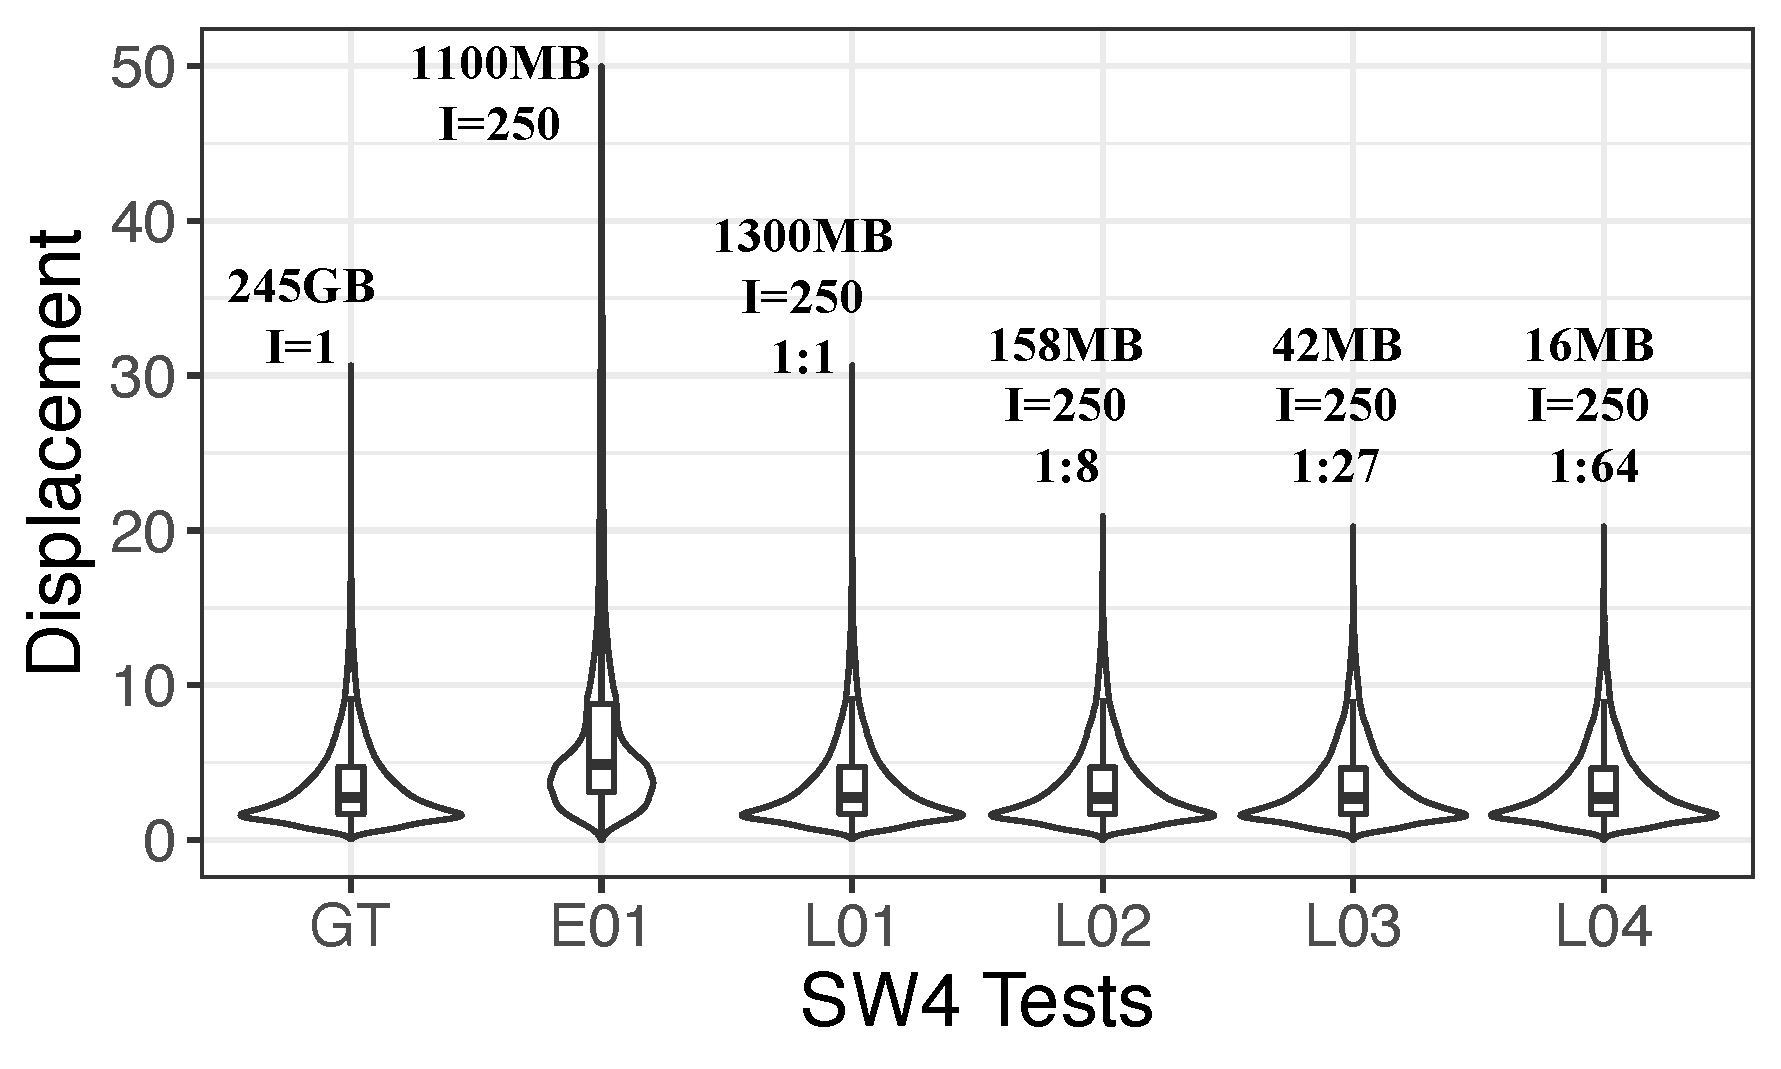
\includegraphics[width=\linewidth]{Images/sw4_violinplot1.pdf}
\vspace{-5mm}
\caption{High displacement near the epicenter.}
\label{fig:epicenter}
\end{subfigure}
\begin{subfigure}{0.495\textwidth}
\centering
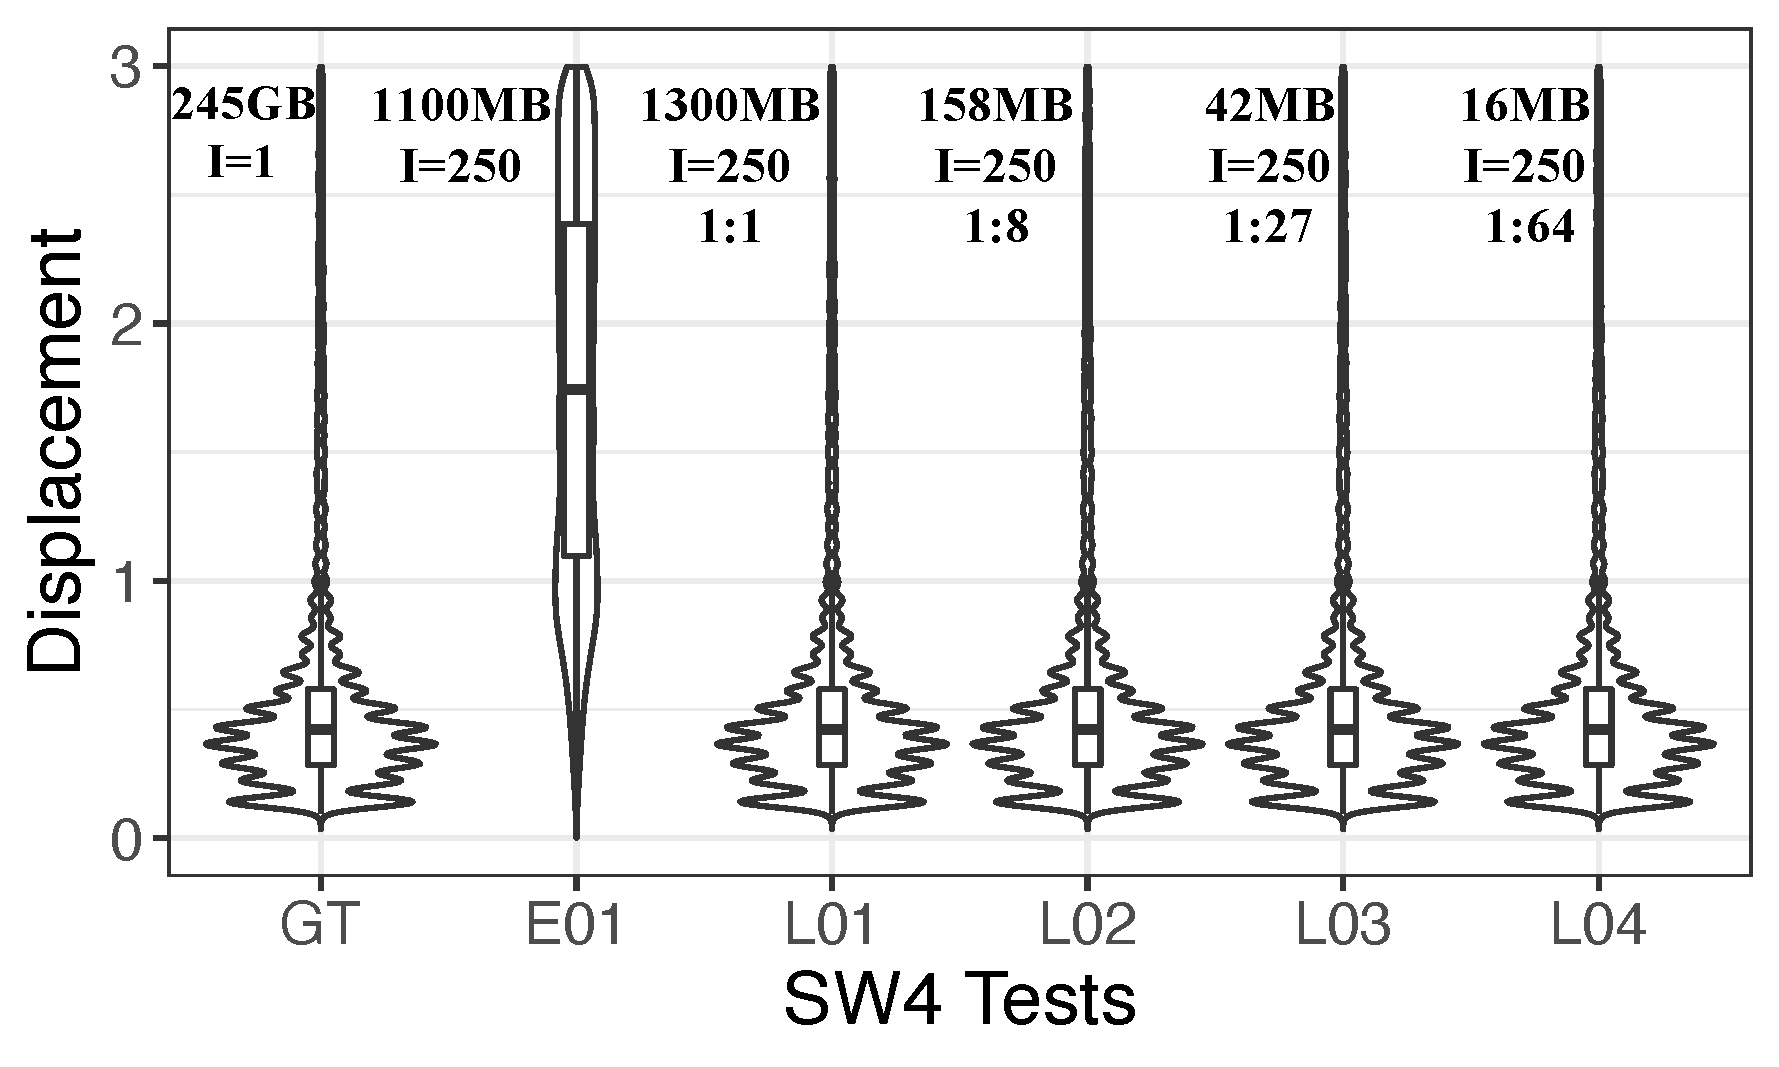
\includegraphics[width=\linewidth]{Images/sw4_violinplot2.pdf}
\vspace{-5mm}
\caption{Low displacement away from the epicenter.}
\label{fig:clusters}
\end{subfigure}
\vspace{-2mm}
\caption{Violin plots of the distribution of particle displacement for the ground truth (GT), one Eulerian configuration and four Lagrangian configurations. The Eulerian configuration, with access to a limited number of time slices, overestimates the displacement. The Lagrangian representation captures displacement in both settings, in regions near and away from the epicenter, accurately.}
\vspace{-5mm}
\label{fig:sw4_violinplot}
\end{figure}

\begin{figure}[!t]
\centering
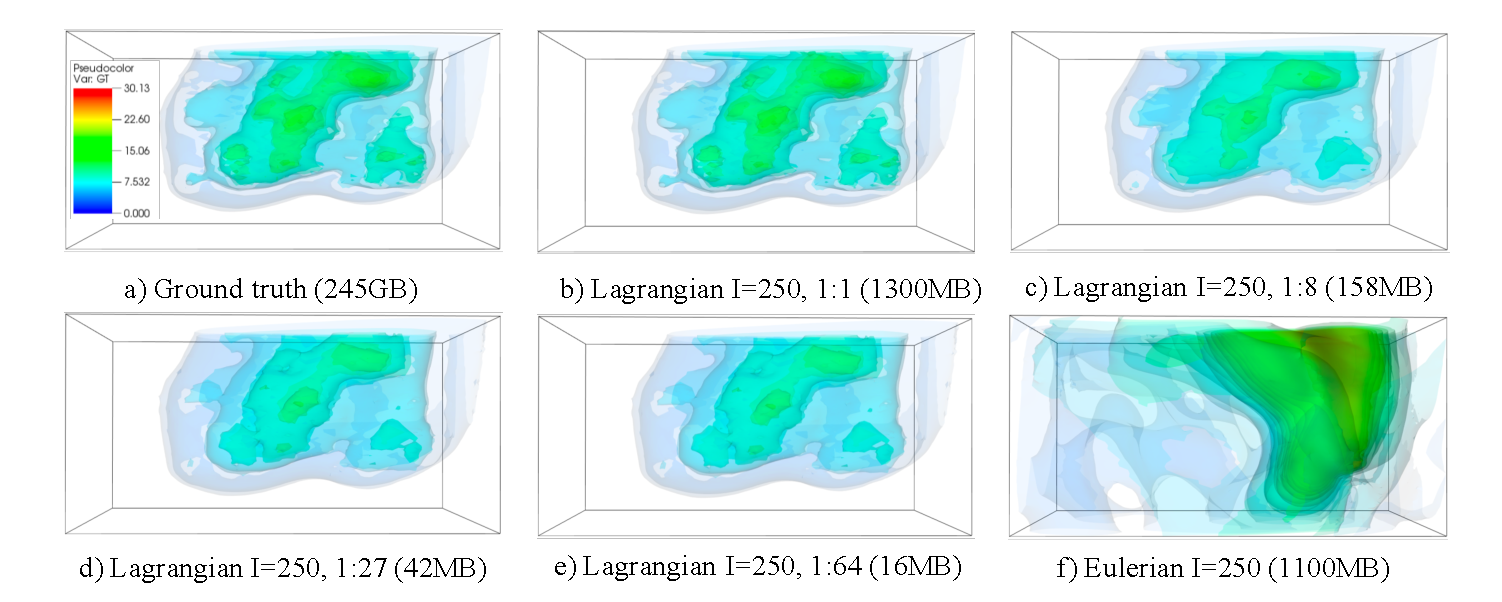
\includegraphics[width=\linewidth, trim={1cm, 0cm, 0.9cm, 0cm}, clip]{Images/sw4_figure_small.pdf}
\vspace{-2mm}
\caption{Visualization of the displacement field derived from reduced Lagrangian representations near the epicenter using multiple isosurfaces. The ground truth is computed using 2000 cycles of the seismic wave propagation simulation. Although at higher data reduction factors regions of high displacement are underestimated, Lagrangian representations are capable of accurately reconstructing the overall feature structure.} 
\vspace{-5mm}
\label{fig:sw4_figure}
\end{figure}


\noindent\textbf{Post Hoc Efficacy}
We studied the reconstruction of the time-varying displacement vector field encoding wave propagation by considering four options for data reduction~(1:1, 1:8, 1:27, 1:64) and 1 option for \textbf{I}~(250).
%
The ground truth was computed using 2000 simulation cycles and required 245 GB.
%
The displacement was highest near the epicenter and reduced as waves propagate further away.
%
For each simulation run, we measured the displacement of 200,000 samples reconstructed near the epicenter (Figure~\ref{fig:epicenter}) and 90,000 samples reconstructed in six regions away from the epicenter (Figure~\ref{fig:clusters}).
%
Here, we directly compare against the distribution of ground truth (GT) displacement.
%
In both cases, Lagrangian representations offered significant data reduction while maintaining high accuracy.
%
We found that as the number of basis trajectories extracted reduces, the displacement for some samples near the epicenter can be underestimated. 
%
In contrast, using a temporally subsampled Eulerian representation (E01) results in significant overestimation of displacement.
%
This result can be expected since temporal subsampling fails to capture the transient nature of wave propagation, whereas Lagrangian representations encoding behavior over an interval of time remain accurate.
%
Compared to Figure~\ref{fig:epicenter}, the ground truth in Figure~\ref{fig:clusters} has smaller displacement and a multimodal distribution that is the result of samples collected from six regions of the domain away from the epicenter. 
%

Figure~\ref{fig:sw4_figure} visualizes the displacement field near the epicenter using multiple semi-opaque isosurfaces.
%
Although the overall structure is well reconstructed using Lagrangian representations, regions of highest displacement can be underestimated as the data reduction factor increases.
%
Overall, we found that Lagrangian representations offer high data reduction options for small loss of accuracy and should be considered more widely for seismic wave propagation vector fields.

%\subsection{Benchmarking Study: Cloverleaf3D}
%\label{sec:cloverleaf3d}

